\documentclass[10pt]{beamer}

% mac版,texShop 中Typeset选择 XeLaTex 

%%%%%%%%%%%%%%%%%%%%%%%%%%%%%%%%%%%%%
\usepackage[slantfont,boldfont]{xeCJK}
%\input{xecjkfonts},CJKtextspaces
\setCJKmainfont{STKaiti}   % STFangsong 设置缺省中文字体
\setCJKmonofont{SimSun}   % 设置等宽字体
\setmainfont{Times} % 英文衬线字体
\setmonofont{Times} % 英文等宽字体
\setsansfont{Times} % 英文无衬线字体
%%%%%%%%%%%%%%%%%%%%%%%%%%%%%%%%%%%%%%

\mode<presentation> {
  %\usetheme{Madrid}
  %\usetheme{Singapore}
  \usetheme{Warsaw}
  \setbeamercovered{transparent}
 % \usefonttheme[onlymath]{serif}  
 \usefonttheme{professionalfonts}%{structurebold}
 % \usefonttheme[onlymath]{structurebold}
  \usecolortheme{rose}
}

\usepackage[english]{babel}
%\usepackage[latin1]{inputenc}

%\usepackage{times}
%\usepackage[T1]{fontenc}


%\usepackage{epsfig}
\usepackage{graphics}
\usepackage{color}
\usepackage{amsmath,amssymb,mathrsfs}
\usepackage{amsfonts,stmaryrd}
%\usepackage{thmmarks}
%\usepackage{}



\newcommand\frakfamily{\usefont{U}{yfrak}{m}{n}}
\DeclareTextFontCommand{\textfrak}{\frakfamily}
\def\diag{\mathrm{diag}}


\title[数值计算方法]{数值计算方法}
\subtitle{-三角插值和快速傅立叶变换}


\subject{Talks}

% If you have a file called "university-logo-filename.xxx", where xxx
% is a graphic format that can be processed by latex or pdflatex,
% resp., then you can add a logo as follows:

% \pgfdeclareimage[height=0.5cm]{university-logo}{university-logo-filename}
% \logo{\pgfuseimage{university-logo}}

%\pgfdeclareimage[height=0.5cm]{university-logo}{ncsu_logo}
%\logo{\pgfuseimage{university-logo}}

% Delete this, if you do not want the table of contents to pop up at
% the beginning of each subsection:
%\AtBeginSubsection[] {
%  \begin{frame}<beamer>
%    \frametitle{Outline}
%    \tableofcontents[currentsection,currentsubsection]
%  \end{frame}
%}

% If you wish to uncover everything in a step-wise fashion, uncomment
% the following command:

% \beamerdefaultoverlayspecification{<+->}


\setbeamertemplate{theorems}[numbered]
\setbeamertemplate{caption}[numbered]


\newtheorem{proposition}[theorem]{Proposition}

%%%%%%%%%%%%%%%%%%%%%%%%%%%
% REMARK-STYLE-ENVIRONMENTS %
%%%%%%%%%%%%%%%%%%%%%%%%%%%
\newcounter{remark}
% \numberwithin{theorem}{section}
\def\openrem#1#2{\refstepcounter{remark}\bigskip

{\noindent\bf#1~\theremark\if#2!{. }\else{ (#2).}\fi}
\it}
\def\thmskip{}
\newenvironment{remark}[1][!]{\openrem{Remark}{#1}}{\thmskip}

%%%%%%%%%%%%%%%%%%%%%%%%%%%%
%% AlGORITHM-STYLE-ENVIRONMENTS %
%%%%%%%%%%%%%%%%%%%%%%%%%%%%
\newcounter{algorithm}
% \numberwithin{theorem}{section}
\def\openalg#1#2{\refstepcounter{algorithm}\bigskip

{\noindent\bf#1~\thealgorithm\if#2!{. }\else{ (#2).}\fi}
\it}
\def\thmskip{}
\newenvironment{algorithm}[1][!]{\openrem{Algorithm}{#1}}{\thmskip}
%
%
%%%%%%%%%%%%%%%%%%%%%%%%%%%%
%% Result-STYLE-ENVIRONMENTS %
%%%%%%%%%%%%%%%%%%%%%%%%%%%%
%\newcounter{result}
%\def\openrem#1#2{\refstepcounter{result}\bigskip
%{\noindent \it \bfseries#1~\theremark\if#2!{. }\else{ (#2). }\fi}}
%\newenvironment{result}[1][!]{\openrem{Result}{#1}}{\qed}




%%%%%%%%%%%%%%%%%%%%%%%%%%%
%Redefine the Symbols%
%%%%%%%%%%%%%%%%%%%%%%%%%%%

\def\mathbi#1{\textbf{\em #1}}

% integrals
\def\dx{\,{\rm d}x}
\def\dxb{\,{\rm d}\boldsymbol{x}}
\def\dy{\,{\rm d}y}
\def\dt{\,{\rm d}t}
\def\ds{\,{\rm d}s}
\def\du{\,{\rm d}u}

\def\dr{\,{\rm d}r}
\def\dtheta{\,{\rm d}\theta}

\def\dd{{\rm d}}

\def\intOm{\int_{\Omega}}
\def\intbOm{\int_{\partial \Omega}}

% differences
\def\Dx{\Delta x}
\def\Dt{\Delta t}
\def\D{\Delta}


% operators
\def\Ls{\mathscr{L}}

% matirices
\def\Js{\mathscr{J}}


%fields%
\def\R{\mathbb{R}}
\def\N{\mathbb{N}}
\def\Z{\mathbb{Z}}

%Spaces%
\def\H{\mathbb{H}}
\def\L{\mathbb{L}}
\def\P{\mathbb{P}}


\def\U{\mathbb{U}}
\def\V{\mathbb{V}}
\def\W{\mathbb{W}}
\def\X{\mathbb{X}}
\def\Y{\mathbb{Y}}

\def\Cinfty{C^\infty}




%vectors%
\def\ab{\boldsymbol{a}}
\def\bb{\boldsymbol{b}}
\def\cb{\boldsymbol{c}}
\def\db{\boldsymbol{d}}
\def\eb{\boldsymbol{e}}
\def\fb{\boldsymbol{f}}
\def\gb{\boldsymbol{g}}
\def\hb{\boldsymbol{h}}
\def\nb{\boldsymbol{n}}
\def\rb{\boldsymbol{r}}
\def\sb{\boldsymbol{s}}


\def\ub{\boldsymbol{u}}
\def\vb{\boldsymbol{v}}
\def\wb{\boldsymbol{w}}
\def\xb{\boldsymbol{x}}
\def\yb{\boldsymbol{y}}
\def\zb{\boldsymbol{z}}

\def\Bb{\boldsymbol{B}}
\def\Cb{\boldsymbol{C}}
\def\Eb{\boldsymbol{E}}
\def\Fb{\boldsymbol{F}}
\def\Ib{\boldsymbol{I}}
\def\Kb{\boldsymbol{K}}
\def\Ob{\boldsymbol{O}}
\def\Qb{\boldsymbol{Q}}
\def\Rb{\boldsymbol{R}}
\def\Sb{\boldsymbol{S}}
\def\Ub{\boldsymbol{U}}
\def\Vb{\boldsymbol{V}}
\def\Wb{\boldsymbol{W}}
\def\Xb{\boldsymbol{X}}
\def\Yb{\boldsymbol{Y}}
\def\Zb{\boldsymbol{Z}}

%domains%
\def\Om{\Omega}
\def\bd{\partial}
\def\bOm{\bar{\Omega}}

%bold symbols%
\def\alphab{\boldsymbol{\alpha}}
\def\phib{\boldsymbol{\varphi}}

%energy%
\def\Jc{\mathcal{J}}
\def\Oc{\mathcal{O}}

%Greeks%
\def\vphi{\varphi}

%Special Functions%
\def\supp{\rm{supp}}
\def\sym{\rm{sym}}

\def\gradu{\nabla u}
\def\gradv{\nabla v}

%Mesh%
\def\Ts{\mathcal{T}}

\def\mach{\rm{mach}}


\begin{document}

\setbeamertemplate{itemize item}[triangle]

\begin{frame}
\titlepage
\end{frame}


\begin{frame}
  \frametitle{本节概要}
  \tableofcontents%[pausesections]
  % You might wish to add the option [pausesections]
%  \begin{itemize}
%  \item 显示Euler法及其误差分析
%  \item Taylor展开法
%  \item 
%  \end{itemize}
\end{frame}

\section{离散傅立叶变换和快速傅立叶变换}

\begin{frame}
\frametitle{离散傅立叶变换}
最小二乘问题可以从两个不同的方面导出。

\vspace{0.2cm}

第一个方面是解线性方程组。我们之前讨论的解线性方程组的问题都一般都假设线性方程组的解存在且唯一,但是在科研和工程实践中,我们有时会遇到方程组个数大于未知数个数的情况,这种情况下方程往往是没有解的。我们解决这个问题的方法一般是在一定的意义下找到近似满足原方程的解,这一般指的就是最小二乘意义下的解。

\vspace{0.2cm}

第二个方面是数据的拟合。我们在插值法一章中严格的要求插值条件满足,也就是插值函数一定要通过所有的插值点。这样个要求一方面会导致插值函数次数升高,另一方面由于数据的测量总会包含误差,因此严格要求插值函数满足插值条件是不必要的。因此,我们往往使用最简单的函数寻找数据点中自变量与因变量之间关系的趋势。

\vspace{0.2cm}
\end{frame}


\begin{frame}
\frametitle{离散傅立叶变换}
设$x = [x_0, \ldots, x_{n-1}]^T$为$n-$维向量,令$\omega = e^{-i \frac{2\pi}{n}}$。
\begin{definition}[离散傅立叶变换]
对于$n-$维向量$x = [x_0, \ldots, x_{n-1}]$,其离散傅立叶变换也是一个$n-$维向量$y = [y_0, \ldots, y_{n-1}]$,满足
\begin{equation}
\label{eq: DFT original}
y_k = \frac{1}{\sqrt{n}} \sum_{j = 0}^{n-1} x_j \omega^{jk},
\end{equation}
其中$\omega = e^{-i \frac{2\pi}{n}}$。
\end{definition}
\end{frame}


\begin{frame}
\frametitle{离散傅立叶变换的矩阵形式}
将上面的定义可以写为矩阵形式
\begin{align*}
\left[ \begin{array}{c}
     y_0 \\ y_1 \\y_2 \\ \vdots \\ y_{n-1}  \end{array} \right]
& \frac{1}{\sqrt{n}} \left[ \begin{array}{ccccc}
     \omega^0    &  \omega^0 &  \omega^0 & \cdots &  \omega^0  \\
     \omega^0    &  \omega^1 &  \omega^2 & \cdots &  \omega^{n-1}  \\
     \omega^0    &  \omega^2 &  \omega^4 & \cdots &  \omega^{2(n-1)}  \\
     \omega^0    &  \omega^3 &  \omega^6 & \cdots &  \omega^{3(n-1)}  \\
     \vdots    &  \vdots & \vdots &\quad &  \vdots  \\
     \omega^0    &  \omega^{n-1} &  \omega^{2(n-1)} & \cdots &  \omega^{(n-1)^2}  \\                   
            \end{array} \right] 
\left[ \begin{array}{c}
     x_0 \\ x_1 \\ x_2 \\ \vdots \\ x_{n-1}  \end{array} \right].
\end{align*}
我们称右端第一个矩阵为傅立叶矩阵
\begin{align}
F_n = & \frac{1}{\sqrt{n}} \left[ \begin{array}{ccccc}
     \omega^0    &  \omega^0 &  \omega^0 & \cdots &  \omega^0  \\
     \omega^0    &  \omega^1 &  \omega^2 & \cdots &  \omega^{n-1}  \\
     \omega^0    &  \omega^2 &  \omega^4 & \cdots &  \omega^{2(n-1)}  \\
     \omega^0    &  \omega^3 &  \omega^6 & \cdots &  \omega^{3(n-1)}  \\
     \vdots    &  \vdots & \vdots &\quad &  \vdots  \\
     \omega^0    &  \omega^{n-1} &  \omega^{2(n-1)} & \cdots &  \omega^{(n-1)^2}  \\                   
            \end{array} \right] .
\end{align}
\end{frame}


\begin{frame}
\frametitle{离散傅立叶逆变换}
对于通过公式\eqref{eq: DFT original}得到的向量$y = [y_0, \ldots, y_{n-1}]$,如果我们在其左侧乘以$F_n$矩阵的逆$F_n^{-1}$,得到的向量就是$x$本身,即$x = F_n^{-1} y$。这个过程称为离散傅立叶逆变换。事实上我们可以证明
\begin{align}
F^{-1}_n = & \frac{1}{\sqrt{n}} \left[ \begin{array}{ccccc}
     \omega^0    &  \omega^0 &  \omega^0 & \cdots &  \omega^0  \\
     \omega^0    &  \omega^{-1} &  \omega^{-2} & \cdots &  \omega^{-(n-1)}  \\
     \omega^0    &  \omega^{-2} &  \omega^{-4} & \cdots &  \omega^{-2(n-1)}  \\
     \omega^0    &  \omega^{-3} &  \omega^{-6} & \cdots &  \omega^{-3(n-1)}  \\
     \vdots    &  \vdots & \vdots &\quad &  \vdots  \\
     \omega^0    &  \omega^{-(n-1)} &  \omega^{-2(n-1)} & \cdots &  \omega^{-(n-1)^2}  \\                   
            \end{array} \right] ,
\end{align}
其中$\omega = e^{-i \frac{2\pi}{n}}$。可以观察到,$F_n^{-1} = \overline{F}_n$。
\end{frame}


\begin{frame}
\frametitle{离散傅立叶变换举例}
\begin{example}
求向量$x = [1,0,-1,0]$的离散傅立叶变换。
\end{example}
由于$x$的维度为4,因此$\omega = e^{-i \frac{\pi}{2}} = \cos(\frac{\pi}{2}) - i \sin(\frac{\pi}{2}) = -i$。利用离散傅立叶变换的公式,得到
\begin{align*}
\left[ \begin{array}{c}
     y_0 \\ y_1 \\y_2  \\ y_{3}  \end{array} \right]
&= \frac{1}{\sqrt{4}} \left[ \begin{array}{cccc}
     1    & 1 & 1  & 1  \\
     1    &  \omega^1 &  \omega^2 &  \omega^{3}  \\
     1    &  \omega^2 &  \omega^4 & \omega^{6}  \\
     1    &  \omega^3 &  \omega^6 & \omega^{9}  \\                 
            \end{array} \right] 
\left[ \begin{array}{c}
     1 \\ 0 \\ -1 \\ 0  \end{array} \right] \nonumber \\
&= \frac{1}{\sqrt{2}} \left[ \begin{array}{cccc}
     1    & 1 & 1  & 1  \\
     1    &  -i &  -1 &  i \\
     1    & -1 &  -1 & i  \\
     1    & -1 & 1  & -1  \\                 
            \end{array} \right] 
\left[ \begin{array}{c}
     1 \\ 0 \\ -1 \\ 0  \end{array} \right] 
= \left[ \begin{array}{c}
     0 \\ 1 \\ 0 \\ 1  \end{array} \right]  .
\end{align*}
\end{frame}


\begin{frame}
\frametitle{离散傅立叶变换的性质和快速傅立叶变换}
\begin{lemma}
令$\{y_k\}_{k = 0}^{n}$是$\{x_j\}_{j = 0}^{n}$的离散傅立叶变换,且$x_j$是实数,则
\begin{enumerate}
\item $y_0$ 是实数;
\item $y_{n-1} = \overline{y}_k, k = 1, \ldots, n-1$。
\end{enumerate}
\end{lemma}

\end{frame}


%%%%%%%%%%%%%%%%%%%%%%%%%%%%%%%%%%%%%%%%%%

\section{三角插值}

\begin{frame}
\frametitle{数据拟合}
考虑数据点$(t_1,y_1), (t_2, y_2), \ldots, (t_m, y_m)$。如果给定一个类型的模型,例如直线$y = c_1 + c_2 t$,我们提出这样一个问题:如何确定参数$c_1, c_2$的值使得这条直线在$2-$范数意义下对这些数据点作了最好的拟合。

\vspace{0.2cm}

如果将上面的语言变为数学语言,那么这等价于:找到参数$c_1, c_2$,使得数据点关于直线$y = c_1 + c_2 t$的残量的平方和最小。可以见下图
\begin{figure}
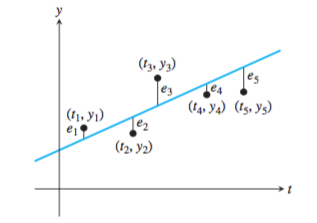
\includegraphics[width=6cm]{figs/4-1-2_Fitting_Data-1} 
%\caption{$f(x) = x^3 + x -1$的图像} 
\end{figure}
\end{frame}



%%%%%%%%%%%%%%%%%%%%%%%%%%%%%%%%%%%%%%%%%%



\section{快速傅立叶变换与信号处理}


\begin{frame}
\frametitle{数据拟合模型}
之前我们考虑了利用多项式模型对数据进行拟合。实际上,我们还有很多其它的数据拟合模型可以选择,这些模型有些是根据数据产生的物理原理得到的,有些是根据经验得到的。
\end{frame}




%%%%%%%%%%%%%%%%%%%%%%%%%%%%%%%%%%%%%%%%%%

\begin{frame}
\frametitle{课后阅读及作业}
[NA] 第4章 4.1.1,4.1.2,4.2 \\
作业:[NA] 4.1:2,3,6,8,9,11;4.2: 1,3,5,6。


\end{frame}

\end{document}

